\documentclass[a4paper,12pt,twoside,openright]{article}
\usepackage[titletoc]{appendix}
\usepackage{textcomp}
\usepackage[pdftex]{color,graphics}
\usepackage{amssymb}
\usepackage{verbatim}
\usepackage{graphicx}
\usepackage{graphics}
\usepackage{amsmath}
\usepackage{rotating}
\usepackage{setspace}
\usepackage{multirow}
\usepackage{array}
\usepackage{hhline}
\usepackage[labelfont={bf}, margin=0.5cm]{caption}
\usepackage{pdflscape}
\usepackage{subcaption}
\usepackage{caption}
\usepackage{xspace}
\usepackage{float}
\usepackage{placeins}
\usepackage{etoolbox}
\usepackage{xkeyval}[2006/11/18]
\usepackage{datetime}
\usepackage[a4paper,inner=1.5cm,outer=1.5cm,top=2.5cm,bottom=2.5cm,pdftex]{geometry}
\usepackage{emptypage}
\usepackage{hyperref}

\hypersetup{
	linktocpage,
    colorlinks = true,
	linkcolor = blue,
	citecolor = red
}

\usepackage{fancyhdr}
\fancyfoot{}
\pagestyle{fancy}
\fancyhead[LO]{\leftmark}
\fancyhead[RE]{\rightmark}
\fancyhead[RO,LE]{\thepage}

\renewcommand{\textfraction}{.05}
\renewcommand{\floatpagefraction}{.40}

\newcommand{\gr}{$\gamma$-ray\xspace}
\newcommand{\grs}{$\gamma$-rays\xspace}

\usepackage{lipsum}% just to automatically generate text

\makeatletter
\newcommand\ackname{Acknowledgements}
\if@titlepage
  \newenvironment{acknowledgements}{%
      \titlepage
      \null\vfil
      \@beginparpenalty\@lowpenalty
      \begin{center}%
        \bfseries \ackname
        \@endparpenalty\@M
      \end{center}}%
     {\par\vfil\null\endtitlepage}
\else
  \newenvironment{acknowledgements}{%
      \if@twocolumn
        \section*{\abstractname}%
      \else
        \small
        \begin{center}%
          {\bfseries \ackname\vspace{-.5em}\vspace{\z@}}%
        \end{center}%
        \quotation
      \fi}
      {\if@twocolumn\else\endquotation\fi}
\fi
\makeatother

\newdateformat{monthyeardate}{%
  \monthname[\THEMONTH], \THEYEAR}

%\textheight 24cm
%\textwidth 16.5cm
%\topmargin -1cm
%\oddsidemargin  0cm
%\evensidemargin 0cm
%\flushbottom

%\usepackage{etoolbox}
%\patchcmd{\chapter}{\thispagestyle{plain}}{\thispagestyle{fancy}}{}{}

\setlength{\headheight}{15pt}


\begin{document}
\begin{center}
\huge \textbf{Are there features in Neutrino Arrival Sky maps that are unique to different number of Sources in the universe?}
\end{center}



\normalsize
ICECUBE is a large scale neurtino located under the South Pole. The experiment consists of 86 strings of light detecting modules drilled 1.5 to 2.5 km below the surface. This resulted in a an observing volume of approximately 100 km$^2$. ICECUBE has a full sky coverage as can even detect neutrinos that have travelled through the Earth. 

\begin{figure}[h]
\centering
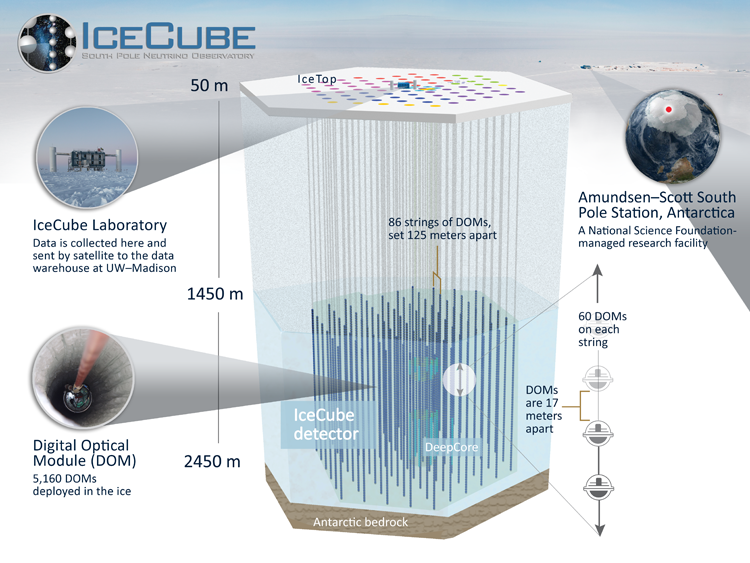
\includegraphics[width=0.7\textwidth]{icecube_detector_sm.png}
\end{figure}


One of the challenges in high energy astrophysics is attributing a source to the detected arrival direction. Narrowing down the type of source/s producing the neutrinos are originating from would greatly help which catalogue to concentrate on when doing source searches. The current method is looking at likely hood probability of events being attributed to a set of sources. Each event is assumed to be independent.
\begin{equation}
\mathcal{L} = \prod_{\mathrm{i}} \sum_{\mathrm{j}} S_{\mathrm{i}}(\mathrm{i} - \mathrm{j})
\end{equation}
Where i is the neutrino event, j is the source and $S$(i-j) is a function that would describe the probability that an event i is associated with a source j.

The main question that we would like to answer is are there features (lumpiness) in Sky maps that can be attributed to different number of sources. We would would like to differentiate between 100 close and strong sources compared to 1 million far but weak sources. Is there added information about how detected events arrive together and test whether or not detected events are truly independent.

\begin{figure}[!h]
\centering
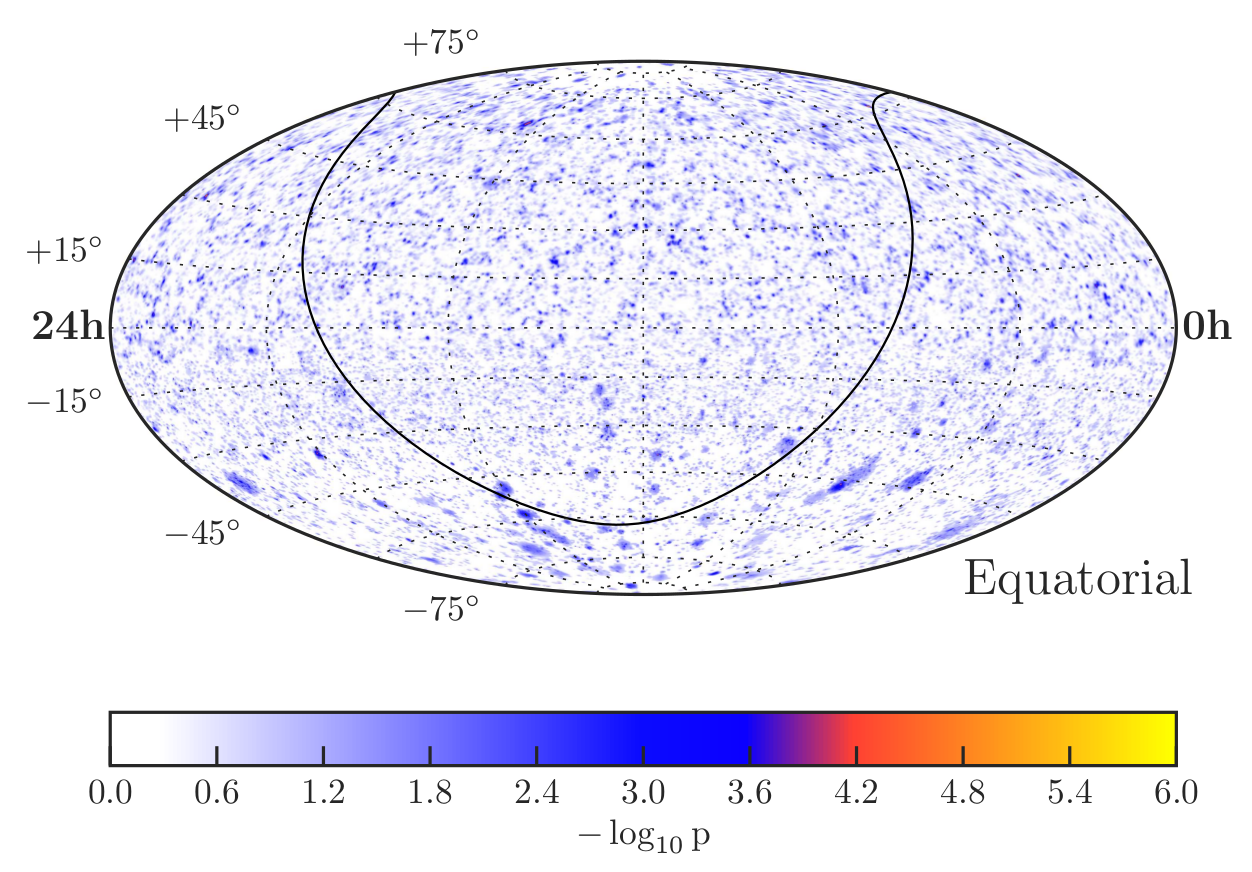
\includegraphics[width=0.8\textwidth]{ICECUBE_eventmap.png}
\caption{All-sky result of the unbinned likelihood maxi-
mization shown in equatorial coordinates (J2000). Shown is
the negative logarithm of the pre-trial p-value, − log 10 p, as-
suming no clustering as null-hypothesis. The Galactic Plane
is shown as black line. Reference - arXiv:1609.04981
}
\end{figure}

\begin{figure}[!h]
\centering
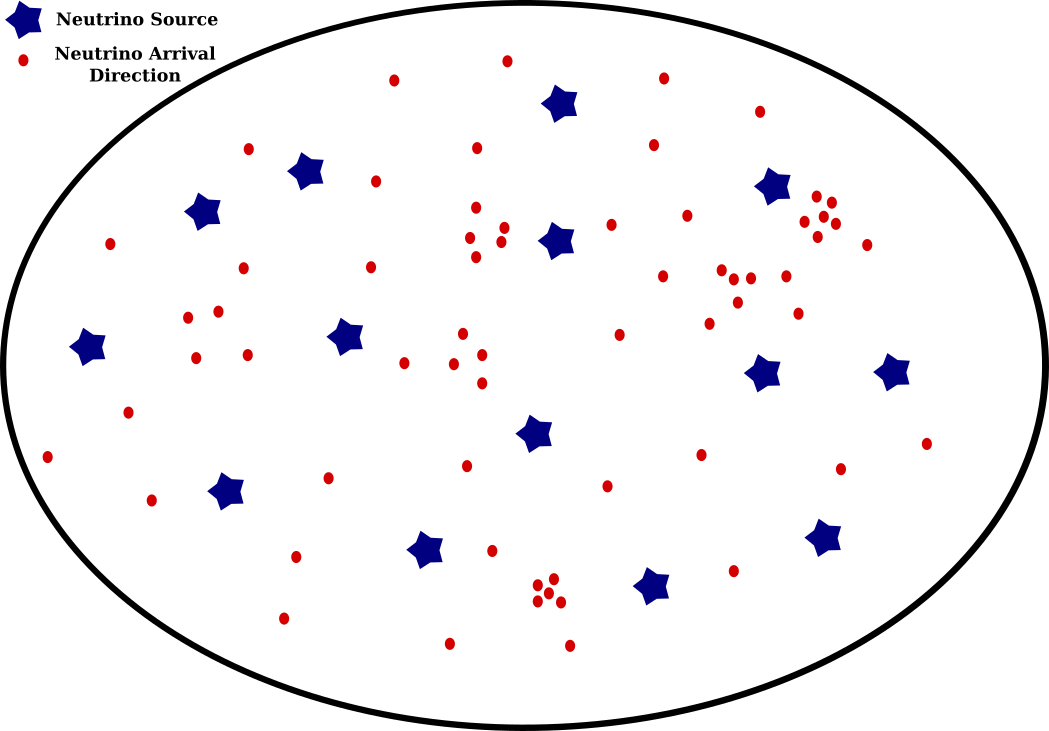
\includegraphics[width=0.6\textwidth]{MockNeutrinoMap.png}
\caption{Diagrammatic example of how sources and arrival directions of neutrinos could be arranged over a sky map. Blue stars represent a neutrino source and red dots represent arrival directions.}
\end{figure}

\end{document}

